\thispagestyle{toanhocvadoisongnone}
\pagestyle{toanhocvadoisong}
\everymath{\color{toanhocdoisong}}
\graphicspath{{../toanhocdoisong/pic/}}
\blfootnote{$^1$\color{toanhocdoisong}Hà Nội.}
\begingroup
\AddToShipoutPicture*{\put(0,616){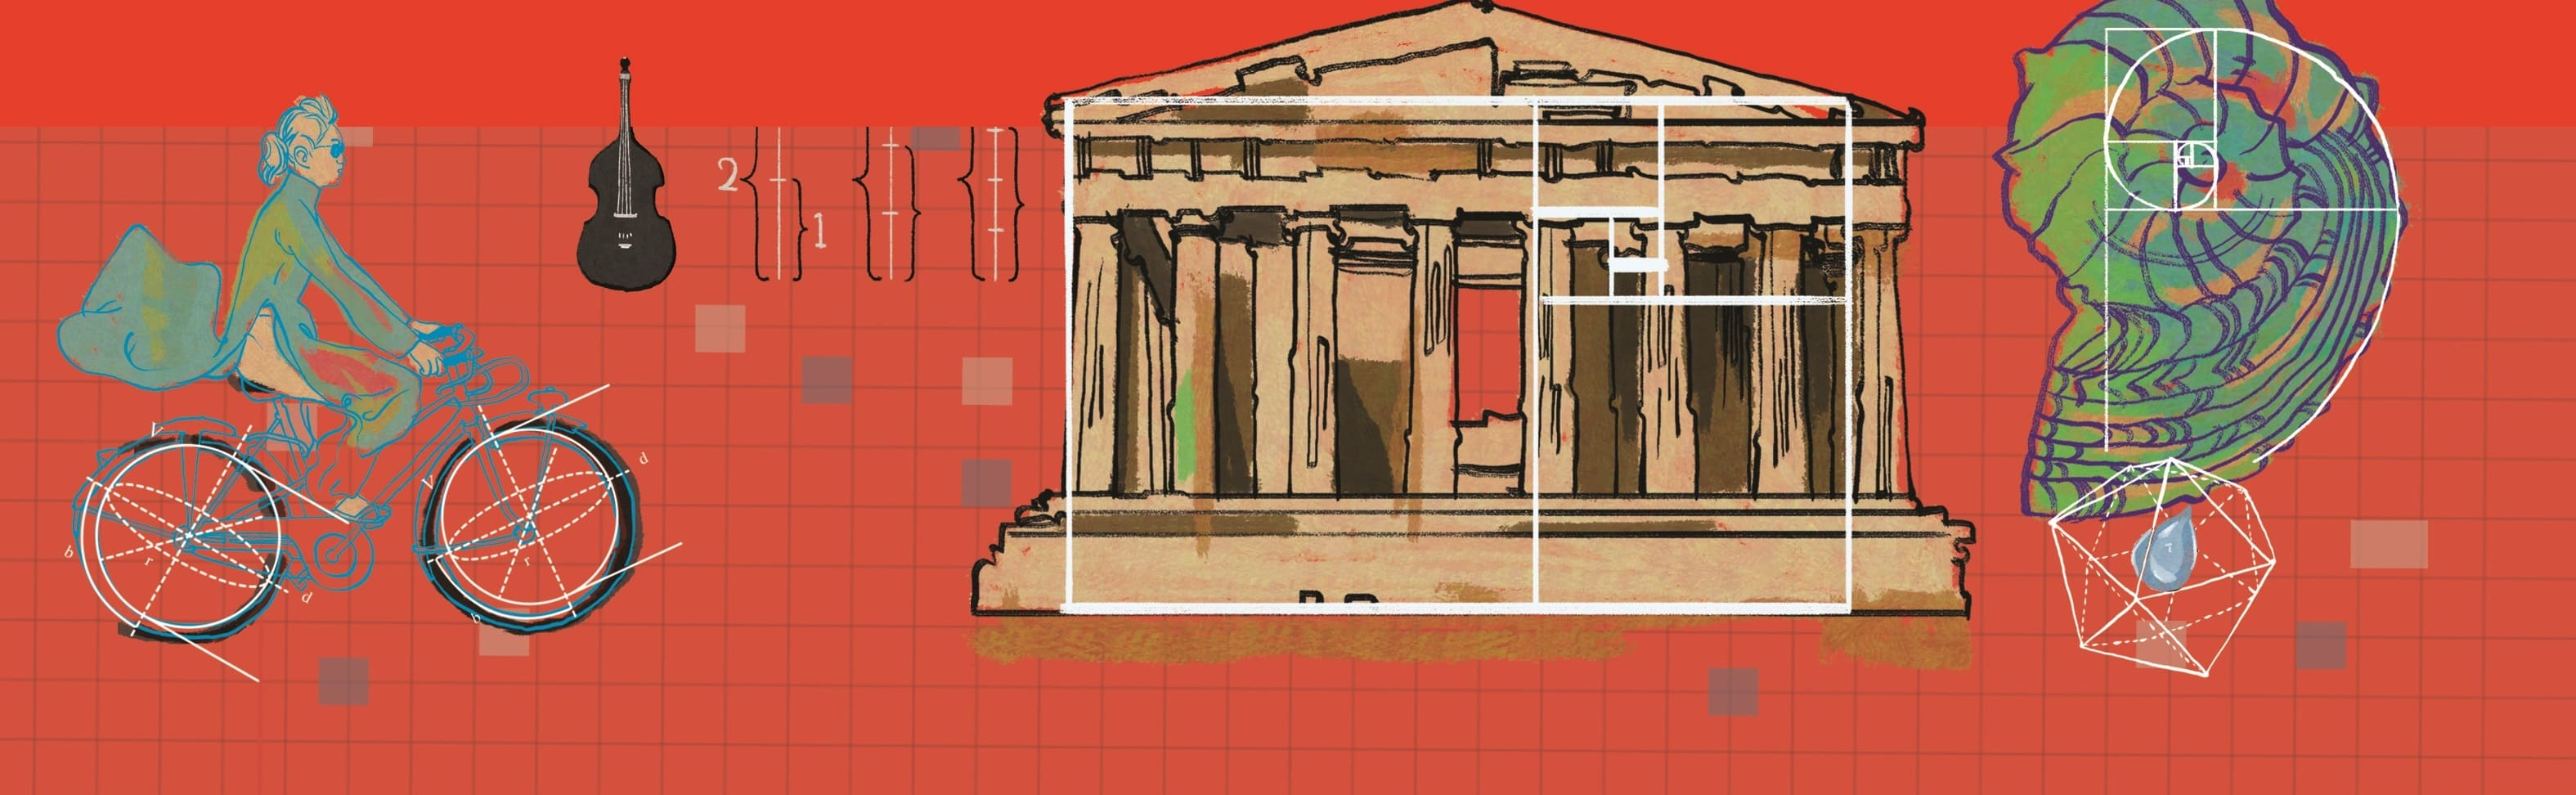
\includegraphics[width=19.3cm]{../bannertoanhocdoisong}}}
\AddToShipoutPicture*{\put(72,524){
\includegraphics[scale=1]{../tieude.pdf}}}
\centering
\endgroup

\vspace*{182pt}

\begin{multicols}{2}
	Có những đường cong tưởng chừng rất xa lạ nhưng lại xuất hiện ở mọi nơi trong đời sống, cả thực lẫn ảo, mà ít người ý thức được sự tồn tại của chúng. Trong bài viết này, chúng ta hãy cùng tìm hiểu về một đường cong như vậy, với tên gọi đường cong Bézier.
	\vskip 0.1cm
	$\pmb{1.}$ \textbf{\color{toanhocdoisong}Bézier, De Casteljau và Bernstein}
	\vskip 0.1cm
	Vào những năm $1950$, với sự phục hồi của nền kinh tế sau chiến tranh thế giới thứ $2$, các hãng xe Pháp bắt đầu nghiên cứu cho ra các sản phẩm mới mang tính thẩm mỹ cao hơn. Tuy nhiên, phương thức tạo khuôn từ mô hình vật lý ban đầu vẫn không khác giai đoạn trước. Sau khi các nhà thiết kế mỹ thuật tạo ra mô hình nhỏ cho một mẫu xe mới, các bề mặt cong sẽ được phóng đại thủ công bằng cách đo đạc các tọa độ từ mô hình này để vẽ lên các bảng thiết kế kích thước thực. Quy trình tạo khuôn yêu cầu quá trình tỉ mỉ và chi tiết đòi hỏi kinh nghiệm cao từ các kỹ sư thực hiện công đoạn này. Sự thiếu rõ ràng và khả năng xảy ra lỗi cao làm cho việc thiết lập mô hình trong sản xuất có thể lặp đi lặp lại nhiều lần dẫn đến việc tăng chi phí và thời gian.
	\vskip 0.1cm
	Mặt khác, cũng vào giai đoạn này, với sự tài trợ của chính phủ Pháp, các máy tính dạng analog bắt đầu xuất hiện trong nhiều ngành công nghiệp. Chúng được nối trực tiếp với các máy thao tác kim loại trong nhà máy. Các thiết bị này sử dụng đầu vào là những tấm bìa đục lỗ để điều chỉnh đường đi cũng như độ sâu của công cụ cắt. Các đường thẳng, đường tròn, parabola và các hình hình học thông thường đều có thể được đưa vào cho máy thao tác một các chính xác. Tuy nhiên, với các dạng đường cong phức tạp hơn, vẫn chưa có một phương thức phù hợp với công nghệ mới này.
	\begin{figure}[H]
		\vspace*{-5pt}
		\centering
		\captionsetup{labelformat= empty, justification=centering}
		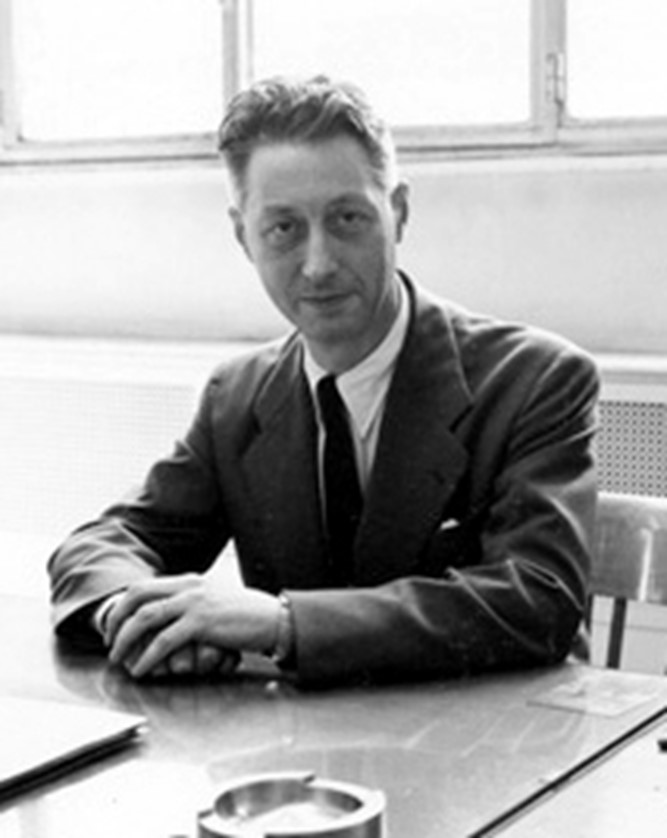
\includegraphics[width= 0.7\linewidth]{1}
		\caption{\small\textit{\color{toanhocdoisong}Pierre Bézier $(1910 - 1999)$.}}
		\vspace*{-10pt}
	\end{figure}	
	Vào đầu những năm $1960$, Pierre Bézier, một kỹ sư tại hãng xe Renault tiến hành tìm phương pháp toán học để giải quyết vấn đề trên. Thay vì dựa vào các kinh nghiệm từ quan sát và thực hành cũng như trí tưởng tượng, việc sản xuất cần được chính xác hóa một cách định lượng. Kết quả từ những nghiên cứu của ông đã cho ra cách xấp xỉ đường cong mà ngày nay được biết đến với tên đường cong Bézier.
	\begin{figure}[H]
		\vspace*{-5pt}
		\centering
		\captionsetup{labelformat= empty, justification=centering}
		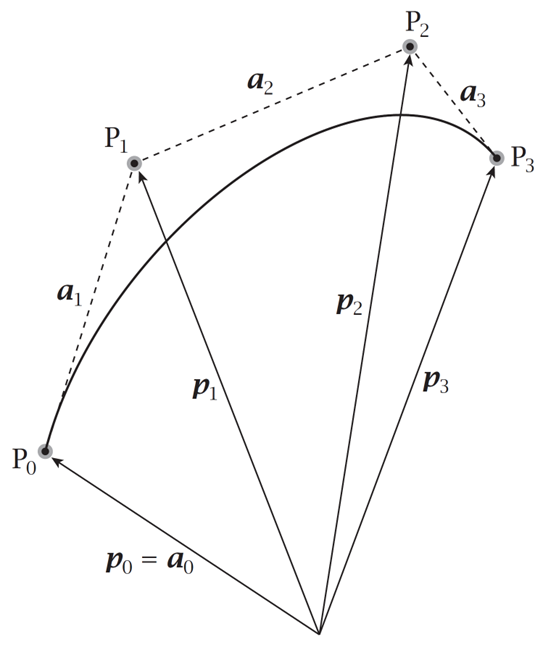
\includegraphics[width= 0.85\linewidth]{2}
		\caption{\small\textit{\color{toanhocdoisong}Hình $1$. Đường cong Bézier được xác định nhờ đường gấp khúc.}}
		\vspace*{-10pt}
	\end{figure}
	Về mặt ý tưởng, đường cong Bézier cho phép ta xấp xỉ một đường cong khác dựa trên một đường gấp khúc. Đồng thời khi điều chỉnh đường gấp khúc này ta cũng có thể thay đổi đường cong được mô tả.
	\vskip 0.1cm
	Ta hãy xét một đường gấp khúc có các đỉnh $P_0,$ $P_1,$ $P_2,$ $P_3$ với các vector tọa độ tương ứng là $\pmb p_0,$ $\pmb p_1,$ $\pmb p_2,$ $\pmb p_3$. Các vector của các đoạn gấp khúc sẽ là:
	\begin{align*}
		\pmb a_1=p_1-p_0,a_2=p_2-p_1,a_3=p_3-p_2.
	\end{align*}
	Vector của mỗi điểm trên đường cong sẽ được biểu diễn theo dạng tham số như sau:
	\begin{align*}
		\pmb{r(t)}=a_0+f_{3,1}(t) \pmb{a_1}+f_{3,2} (t) \pmb{a_2}+f_{3,3} (t) \pmb{a_3}
	\end{align*}
	với $\pmb a_0=p_0$ và $f_{3,i}$ là các hàm số của $t$ trong khoảng $[0,1]$.
	\vskip 0.1cm 
	Ta muốn đường cong tham số của ta có hai đầu trùng với đường cong thực tế, tức là:
	\begin{align*}
		\pmb r(0)=p_0,r(1)=p_3. 
	\end{align*}
	Thay vào biểu thức của $\pmb r(t)$, ta được: $f_{3,1} (0)=f_{3,2} (0)=f_{3,3} (0)=0$ và $f_{3,1} (1)=f_{3,2}(1)=f_{3,3}(1)=1$.
	\vskip 0.1cm
	Tiếp theo, ta muốn rằng tiếp tuyến tại $P_0$ và $P_3$ sẽ cùng phương và chiều với các vector $\pmb a_1$ và $\pmb a_3$. Lấy đạo hàm của $\pmb r(t)$ theo $t$ ta có:
	\begin{align*}
		\pmb{r' (t)}=f_{3,1}' (t) \pmb{a_1}+f_{3,2}' (t) \pmb{a_3}+f_{3,3}' (t) \pmb{a_3}.
	\end{align*}
	Điều kiện về tiếp tuyến sẽ cho ta:
	\begin{align*}
		\pmb{r'(0)}&=f_{3,1}' (0) \pmb{a_1}+f_{3,2}' (0) \pmb{a_2}+f_{3,3}'(0) \pmb{a_3}\\
		&=ka_1\\
		\pmb{r'(1)}&=f_{3,1}' (1) \pmb{a_1}+f_{3,2}' (1) \pmb{a_2}+f_{3,3}'(1) \pmb{a_3}\\
		&=k\pmb{a_3}
	\end{align*}
	tương đương với $f_{3,2}' (0)=f_{3,3}' (0) = f_{3,1}' (1)=f_{3,2}' (1)=0$.
	\vskip 0.1cm
	Ta cũng muốn rằng đạo hàm cấp hai $\pmb{r''(t)}=f_{3,1}'' (t) \pmb{a_1}+f_{3,2}'' (t) \pmb{a_2}+f_{3,3}'' (t) \pmb{a_3}$ chỉ phụ thuộc vào ${\pmb a_1,a_2}$ tại $P_0$ và ${\pmb a_2,a_3}$ tại $P_3$. Để thỏa mãn điều kiện này $f_{3,3}'' (0)=f_{3,1}'' (1)=0$.
	\vskip 0.1cm
	Bezier chọn các hàm $f$ là các hàm đa thức bậc $3$:
	\begin{align*}
		f_{3,i}(t)=\alpha_i t^3 + \beta_i t^2+\gamma_i t + \delta_i,1 \le i \le 3.
	\end{align*}
	Thay vào các điều kiện ở trên và giải hệ phương trình tuyến tính ta được:
	\begin{align*}
		&f_{3,1} (t)=t^3-3t^2+3t\\
		&f_{3,2} (t)=-2t^3+3t^2\\
		&f_{3,3} (t)=t^3.
	\end{align*}
	Khi đó:
	\begin{align*}
		\pmb{r(t)}=\,&\pmb{a_0}+(t^3-3t^2+3t) \pmb{a_1}\\
		&+(-2t^3+3t^2 ) \pmb{a_2}+t^3 a_3, \,\,\,0 \le t \le 1.
	\end{align*}
	Phương trình đường cong theo tham số này cho phép ta điều chỉnh hình dạng của đường cong bằng cách thay đổi các vector $\pmb a_0,$ $\pmb a_1,$ $\pmb a_2,$ $\pmb a_3$. Đường cong Bezier cũng có thể được mở rộng bằng cách sử dụng các đa thức với bậc lớn hơn $3$ nhưng trong thực tế việc này là không cần thiết. Thậm chí trong một số trường hợp đơn giản hơn, người ta chỉ dùng đường cong Bezier bậc $2$:
	\begin{align*}
		\pmb{r(t)}=\pmb{a_0}+(-t^2+2t) \pmb{a_1}+t^2 \pmb{a_2}.
	\end{align*}
	Bezier đã phát triển phương pháp mô tả đường cong trên của mình thành hệ thống UNISURF phục vụ cho công việc sản xuất ô tô. Thay vì những mô tả phức tạp, với mỗi đoạn cong, ta chỉ cần lưu tọa độ của $4$ điểm mà thôi, giúp cho việc số hóa đường cong trở nên đơn giản hơn rất nhiều. Tuy nhiên phải đến năm $1966$, khi Renault ký thỏa thuận hợp tác với một hãng xe nổi tiếng khác là Peugeot, phần mềm này mới bắt đầu được các kỹ sư sử dụng. Năm $1968$ đánh dấu sự ra đời của mẫu xe Peugeot $204$, chiếc xe đầu tiên có toàn bộ vỏ xe được xây dựng sử dụng phần mềm máy tính. Sự kiện này có ý nghĩa quan trọng là cột mốc bắt đầu vai trò của CAD (Computer Aided Design -- thiết kế có máy tính hỗ trợ) trong các ngành công nghiệp.
	\begin{figure}[H]
		\vspace*{-5pt}
		\centering
		\captionsetup{labelformat= empty, justification=centering}
		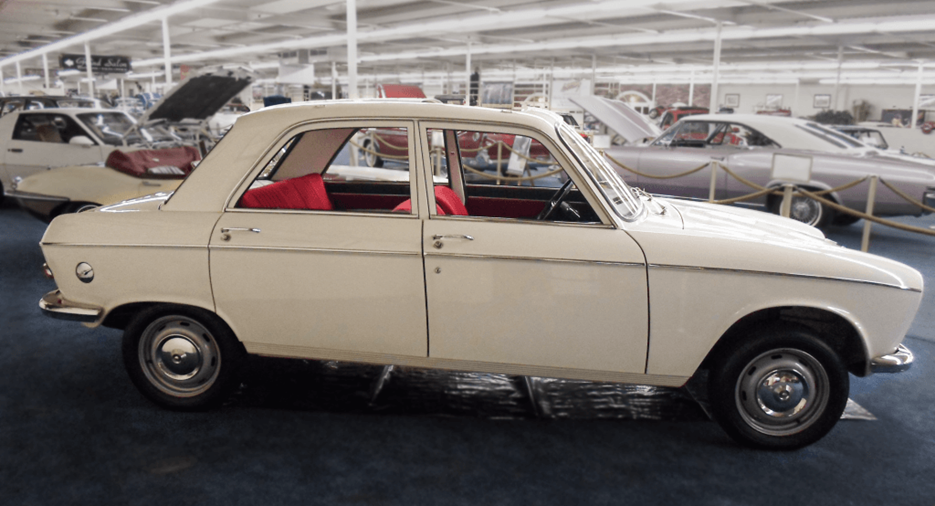
\includegraphics[width= 1\linewidth]{3}
		\caption{\small\textit{\color{toanhocdoisong}Hình $2$. Mẫu xe Peugeot $204$ ra đời năm $1968$.}}
		\vspace*{-10pt}
	\end{figure}
	\vskip 0.1cm
	\PIbox{Bézier từng kể lại rằng, một nhân tố giúp ông thuyết phục thành công mọi người sử dụng phương pháp của mình là việc gán các kết quả toán học cho giáo sư Onésimer Durand, một nhân vật giả tưởng ông tự bịa ra. Điều này giúp mọi người cảm thấy tin tưởng nhiều hơn vào các kết quả của Bézier. Nhiều thập kỉ sau, Bézier khi đi giảng bài vẫn được hỏi rằng giáo sư Durand là ai và giảng dạy ở đâu!}
	\vskip 0.1cm
	Về mặt lịch sử, đường cong Bézier đã được khám phá trước đó không lâu bởi De Casteljau, một kỹ sư ở hãng xe Citroën cũng của Pháp. Công trình này được ông công bố nội bộ năm $1963$. Tuy nhiên, do hãng coi đây là một bí mật công nghiệp, nó đã không được công bố ra bên ngoài cho đến tận năm $1975$.
	\vskip 0.1cm
	Thay vì sử dụng các vector như Bézier, De Casteljau xấp xỉ các đường cong dựa trên các điểm cực. Giả sử một đường cong có hai đầu ở $P_0$ và $P_2$. Một điểm $P_1$ được sử dụng để làm điểm điều khiển. Trên $P_0 P_1$ lấy điểm $Q_0$sao cho $\dfrac{P_0Q_0}{P_0P_1} = k$ Tương tự, trên $P_1 P_2$ lấy điểm $Q_1$ sao cho $\frac{P_1 Q_1}{P_1 P_2}$ cũng bằng $k$. Trên $Q_0 Q_1$ ta lại lấy điểm $R$ sao cho $\dfrac{Q_0 R}{Q_0 Q_1} = k$. Từ tọa độ của $P_0,$ $P_1,$ $P_2$ có thể dễ dàng tính được tọa độ của $Q_0,$ $Q_1$ và $R$ bằng các công thức hình học giải tích. $R$ sẽ là một điểm nằm trên đường cong ta cần mô tả. Tiếp đó, các bộ ba điểm $P_0,$ $Q_0,$ $R$ và $R,$ $Q_1,$ $P_2$ lại cho ta $2$ điểm tiếp theo thuộc đường cong. Lặp lại quá trình này cho đến khi được số lượng điểm nằm trên đường cong đủ dày đặc, ta có thể nối chúng bằng các đoạn thẳng để xấp xỉ đường cong. Bạn đọc có thể tự chứng minh để thấy rằng các điểm được xác định bằng thuật toán trên nằm trên một đường cong Bézier bậc $2$. Khi ta di chuyển các điểm $P_0,$ $P_1$  và $P_2$, ta có thể thay đổi được hình dạng của đường cong theo ý muốn.
	\begin{figure}[H]
		\vspace*{-5pt}
		\centering
		\captionsetup{labelformat= empty, justification=centering}
		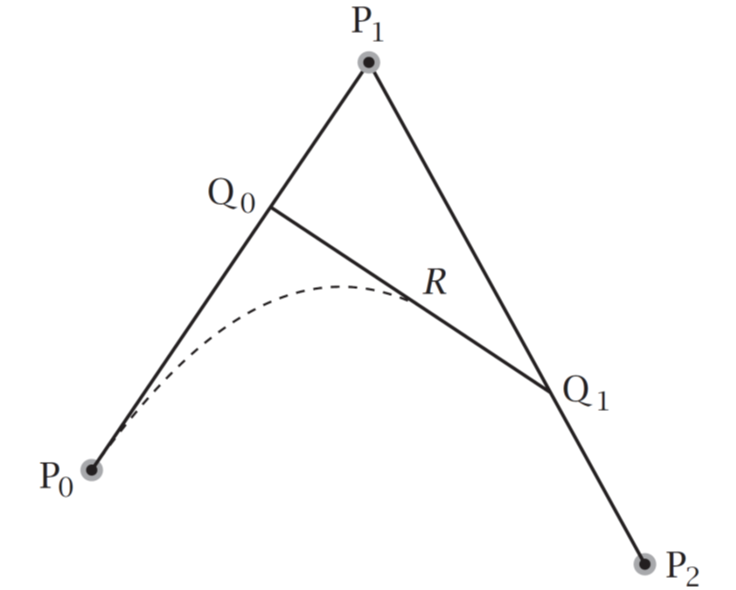
\includegraphics[width= 0.9\linewidth]{4}
		\caption{\small\textit{\color{toanhocdoisong}Hình $3$. Thuật toán De Casteljau.}}
		\vspace*{-5pt}
	\end{figure}
	Do De Casteljau phát hiện ra trước nhưng không được đặt tên cho đường cong, người ta đã bù đắp bằng cách đặt tên thuật toán tách đường cong trên là thuật toán De Casteljau. Thuật toán De Casteljau với $k=0,5$ có thể được cài đặt hiệu quả trên các máy tính điện tử do việc chia một số cho $2$ là rất dễ dàng với hệ cơ số nhị phân.
	\vskip 0.1cm
	Đường cong Bézier còn có thể được mở rộng cho không gian $3$ chiều. Khi đó ta sẽ có mặt cong Bézier.
	\begin{figure}[H]
		\vspace*{-5pt}
		\centering
		\captionsetup{labelformat= empty, justification=centering}
		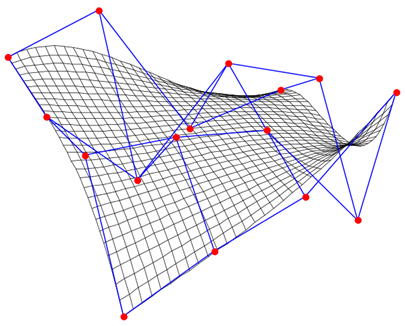
\includegraphics[width= 1\linewidth]{5}
		\caption{\small\textit{\color{toanhocdoisong}Hình $4$. Mặt cong Bézier trong không gian $3$ chiều.}}
		\vspace*{-10pt}
	\end{figure}
	\textbf{\color{toanhocdoisong}Đường cong Bézier và font chữ máy tính}
	\vskip 0.1cm
	Việc hiển thị các font chữ khi soạn thảo văn bản trên máy tính cũng như khi in ấn từ máy tính là một vấn đề tưởng đơn giản nhưng lại phức tạp. Vào thời ban đầu của máy tính, các font được lưu dưới dạng bitmap, với các kích cỡ font khác nhau, ta cần các bitmap với độ phân giải khác nhau, rất tốn kém và không hiệu quả.
	\vskip 0.1cm
	Đến năm $1985$, John Warnock, người sáng lập ra công ty Adobe, đã đưa ra một giải pháp mới. Ông đã phát triển một ngôn ngữ lập trình tên gọi PostScript để có thể xây dựng trang văn bản dựa trên các cấu trúc toán học. Trong đó, các font chữ được lưu dưới dạng font vector, dạng font mà sau này cả Apple lẫn Microsoft đều sử dụng cho các thế hệ font chữ sau này. Với những thành phần của font chữ là dạng đường cong, đường cong Bézier bậc $3$ được sử dụng để lưu trữ chúng trong máy tính. Ví dụ như với chữ O ở bên dưới, với mỗi đoạn cong giữa hai điểm được đánh dấu liên tiếp, người ta cần lưu $4$ tọa độ gồm tọa độ của hai điểm được đánh dấu và tọa độ của hai điểm còn lại để biểu diễn đoạn cong này dưới dạng đường cong Bezier.
	\vskip 0.1cm
	Đường cong Bézier cũng trở thành công cụ chính trong Illustrator, một phần mềm khác của Adobe. Thay vì các thao tác phức tạp, những người thiết kế đồ họa chỉ cần nhấn chuột vài lần để tạo một đường cong trong phần mềm. Việc này đã thay đổi hoàn toàn ngành công nghiệp thiết kế đồ họa.
	\begin{figure}[H]
		\vspace*{-5pt}
		\centering
		\captionsetup{labelformat= empty, justification=centering}
		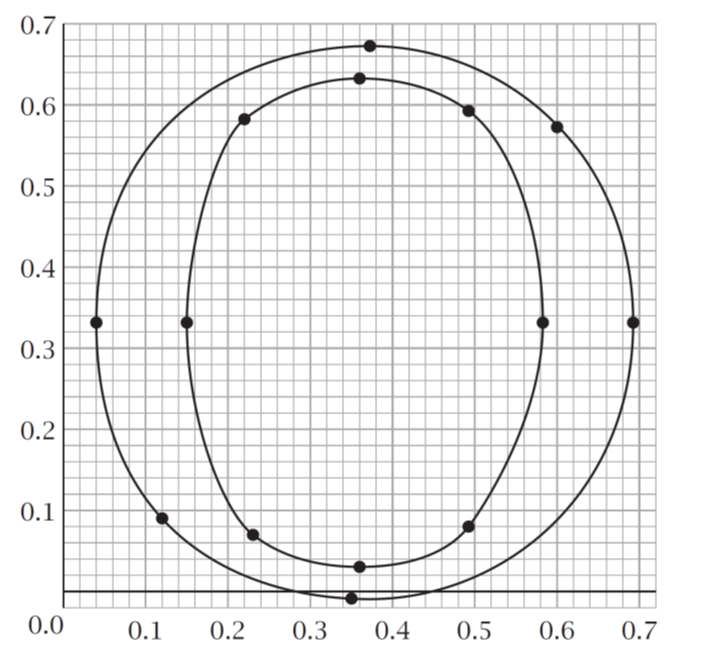
\includegraphics[width= 1\linewidth]{6}
		%		\caption{\small\textit{\color{}}}
		\vspace*{-15pt}
	\end{figure}
	$\pmb2.$ \textbf{\color{toanhocdoisong}Sơ lược về đa thức Bernstein}
	\vskip 0.1cm
	Nếu viết đường cong Bézier bậc $3$ theo tọa độ của các điểm xác định nó (thay vì các vector $\pmb a_i$), ta được phương trình:
	\begin{align*}
		\pmb{r(t){}= &(1-t)^3 \pmb{p_0}+3t(1-t)^2 \pmb{p_1}\\
			&+3t^2 (1-t) \pmb{p_2}+t^3 \pmb{p_3}.
		\end{align*}
		Các đa thức $(1-t)^3,3t(1-t)^2,3t^2 (1-t)$ và $t^3$ có thể được coi là trọng số ứng với tọa độ của mỗi điểm trong biểu diễn của đường cong. Bạn đọc với trực giác toán học tốt sẽ nhận ngay thấy chúng là các đa thức thành phần khi ta tiến hành khai triển $\left(t+(1-t)\right)^3$.
		\vskip 0.1cm
		Các đa thức dạng này còn được gọi là các đa thức Bernstein:
		\begin{align*}
			B_i^n (t)&= \left(\begin{array}{l}
				n\\
				i
			\end{array}\right)t^i (1-t)^(n-i),\\
			&1 \le i \le n,0 \le t \le 1.
		\end{align*}
		Các đa thức Bernstein được suy ra từ biến đổi sau:
		\begin{align*}
			1 &= 1^n = \left(t + (1-t)\right) \\
			&= \sum\limits_{i = 0}^n {\left( \begin{array}{l}
					n\\
					i
				\end{array} \right){t^i}{{(1 - t)}^{n - i}} = } \sum\limits_{i = 0}^n {B_i^n(t).}
		\end{align*}
		Chúng được đặt tên theo nhà toán học Liên Xô Sergei Bernstein. Ông là một nhà toán học có nhiều đóng góp về vấn đề xấp xỉ hàm số. Ta luôn có thể biểu diễn một đa thức bất kì dưới dạng tổ hợp tuyến tính của các đa thức Bernstein. Theo thuật ngữ trong đại số tuyến tính, các đa thức này tạo thành một cơ sở của không gian vector các đa thức.
		\begin{figure}[H]
			\vspace*{-5pt}
			\centering
			\captionsetup{labelformat= empty, justification=centering}
			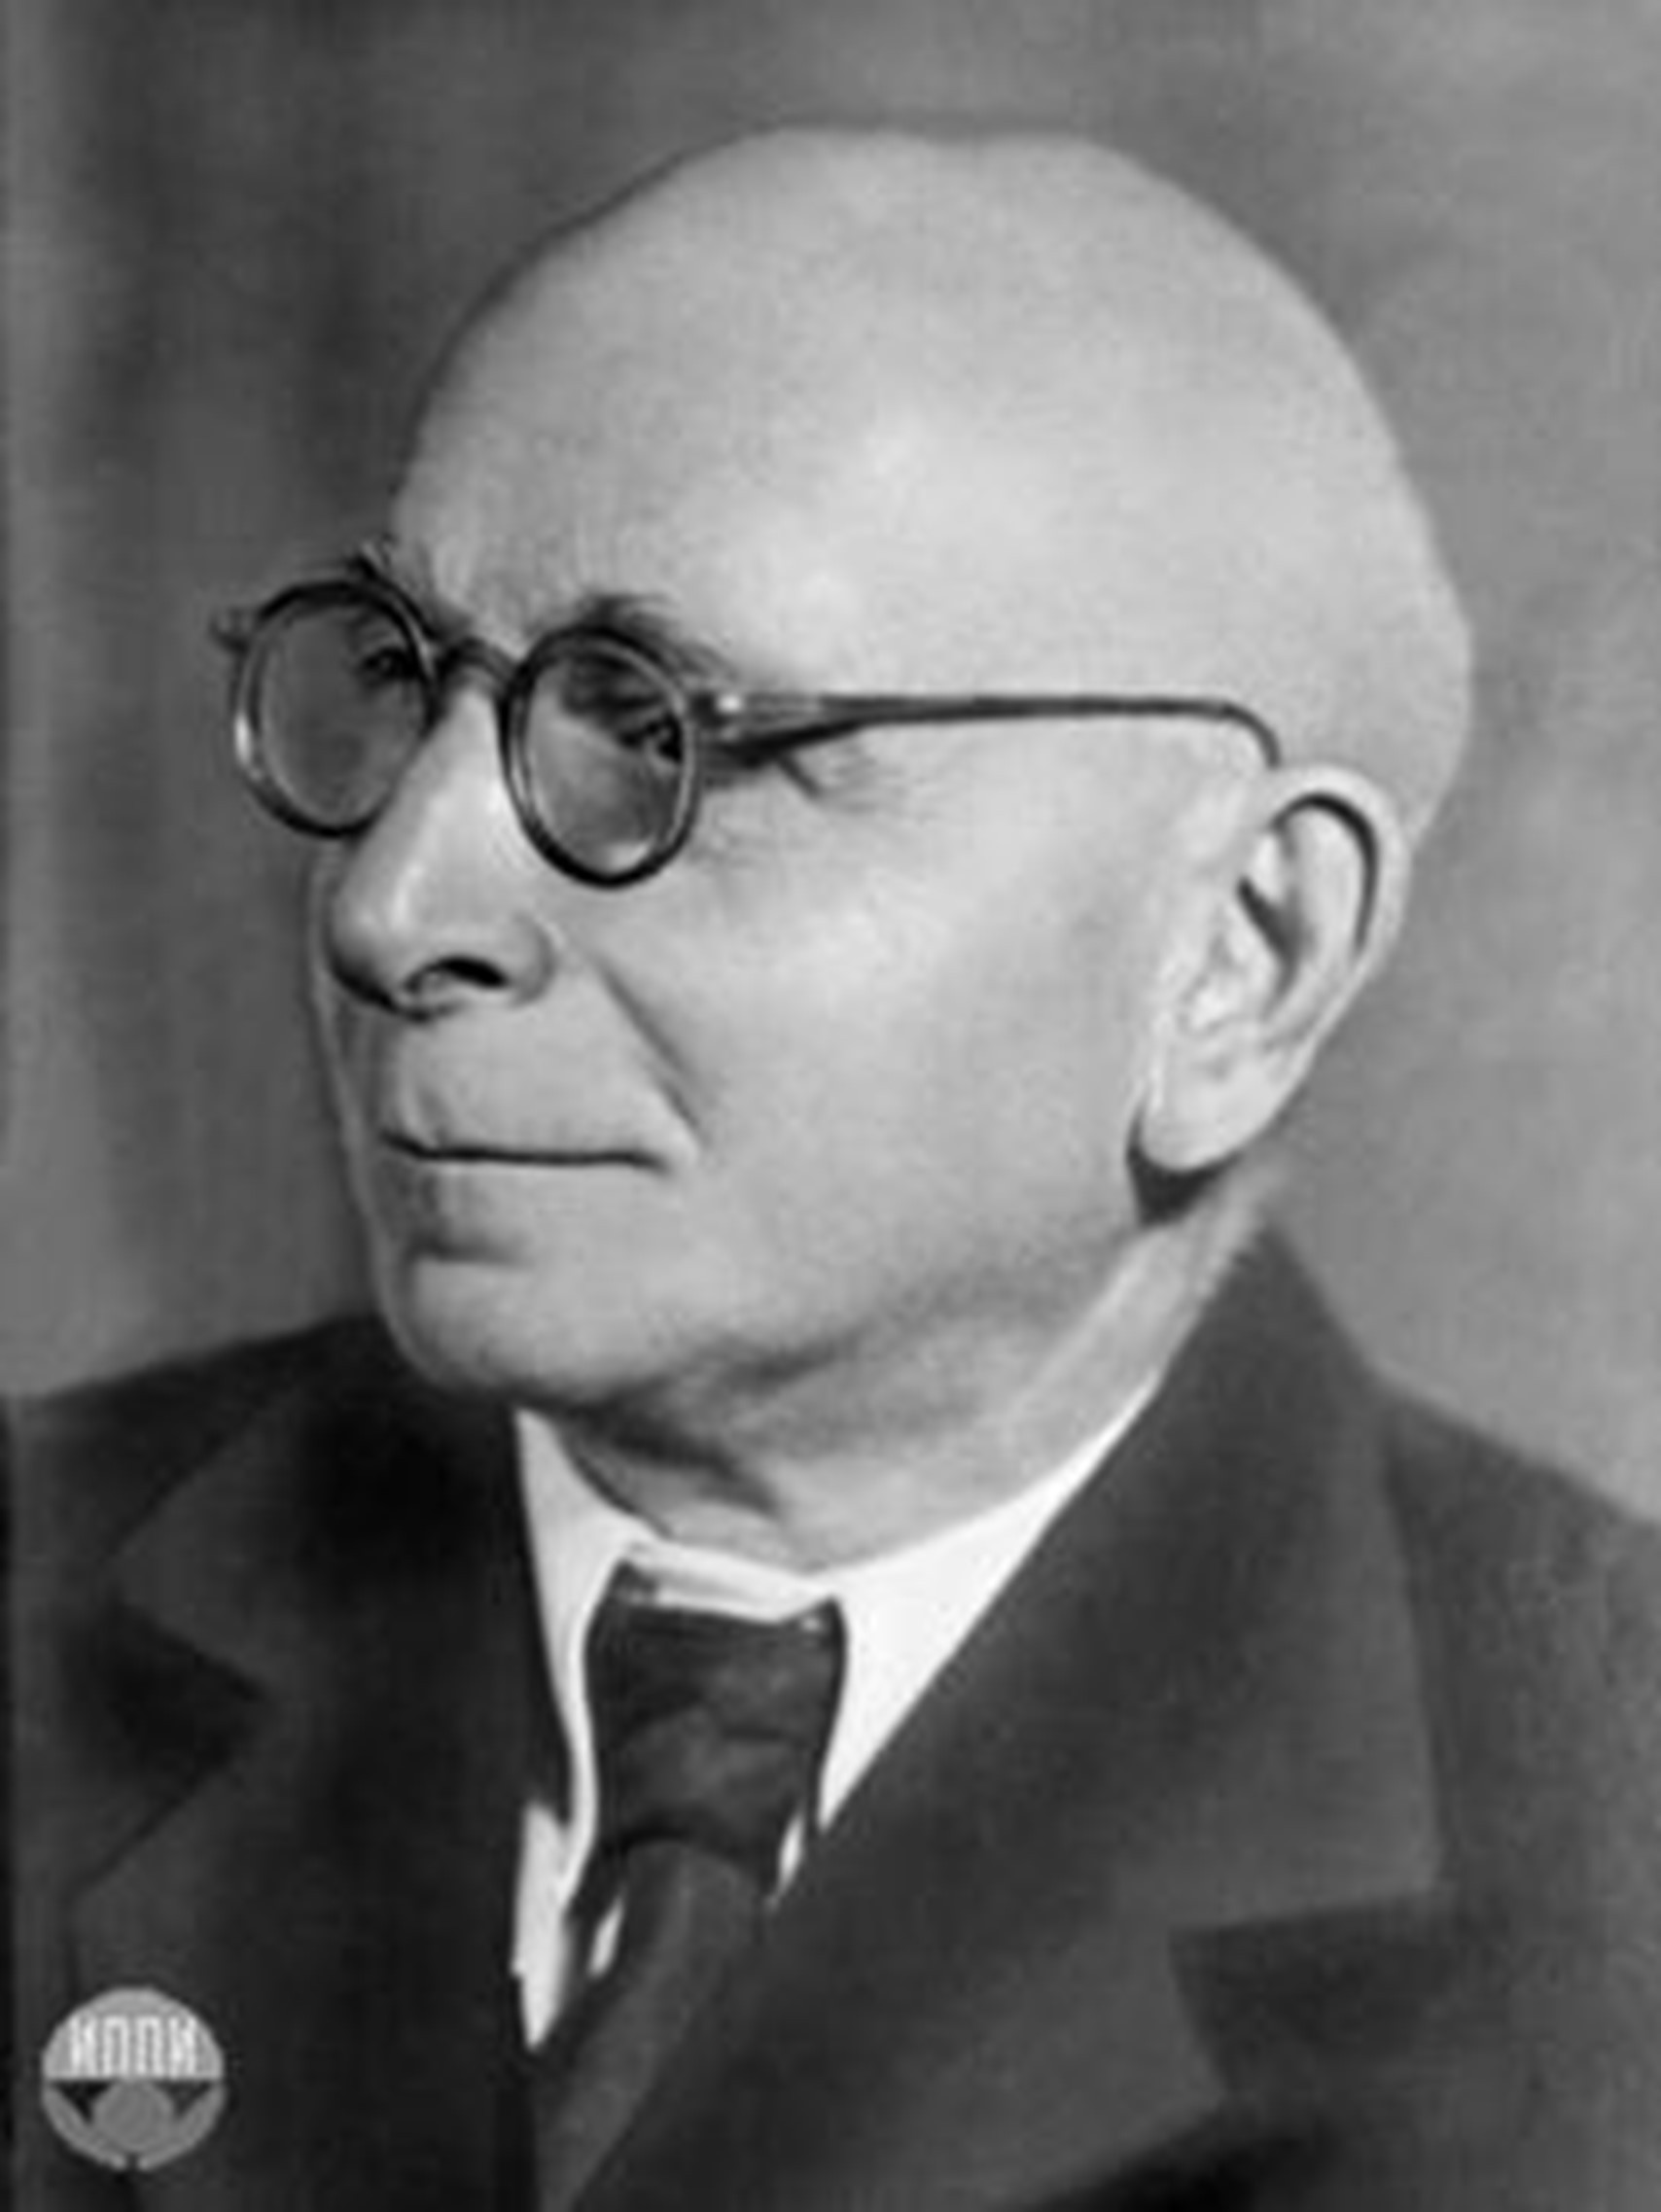
\includegraphics[width= 0.6\linewidth]{7}
			\caption{\small\textit{\color{toanhocdoisong}Sergei Natanovich Bernstein $(1880-1968)$.}}
			\vspace*{-10pt}
		\end{figure}
		Bernstein đã sử dụng các đa thức mang tên mình để chứng minh định lí xấp xỉ Weierstrass: ``các đa thức với bậc đủ cao có thể xấp xỉ bất cứ hàm số liên tục nào trên một khoảng hữu hạn''. Ông đã chứng minh rằng:
		\begin{align*}
			\mathop {\lim }\limits_{n \to \infty } {B_n}(f,t) = f(t)
		\end{align*}
		với $B_n(f,t) = \sum\limits_{i = 0}^n {f\left( {\frac{i}{n}} \right)B_i^n(t)}$ trên khoảng $[0,1]$ (chứng minh này được trình bày ở phần phụ lục). Do biến đổi $t \to \dfrac{t-a}{b-a}ra$ cũng biến đổi $[a,b] \to [0,1]$ nên định lý được chứng minh.
		\vskip 0.1cm
		Tuy rằng tốc độ hội tụ của hàm đa thức $B_n$ rất chậm, trong thực tế các đa thức Bernstein bậc $2$ hoặc bậc $3$ thường đã đủ để thỏa mãn các nhu cầu ứng dụng, ví dụ như trường hợp đường cong Bézier. Bản thân De Casteljau cũng đã tiến hành xây dựng nghiên cứu của mình dựa trên lý thuyết về đa thức Bernstein. Có thể thấy rằng những nghiên cứu toán học tưởng như trừu tượng lại nhiều lúc tạo cơ sở cho những ứng dụng thực tiễn đầy thú vị.
		\vskip 0.1cm
		\textbf{\color{toanhocdoisong}Hàm spline}
		\begin{figure}[H]
			\vspace*{-5pt}
			\centering
			\captionsetup{labelformat= empty, justification=centering}
			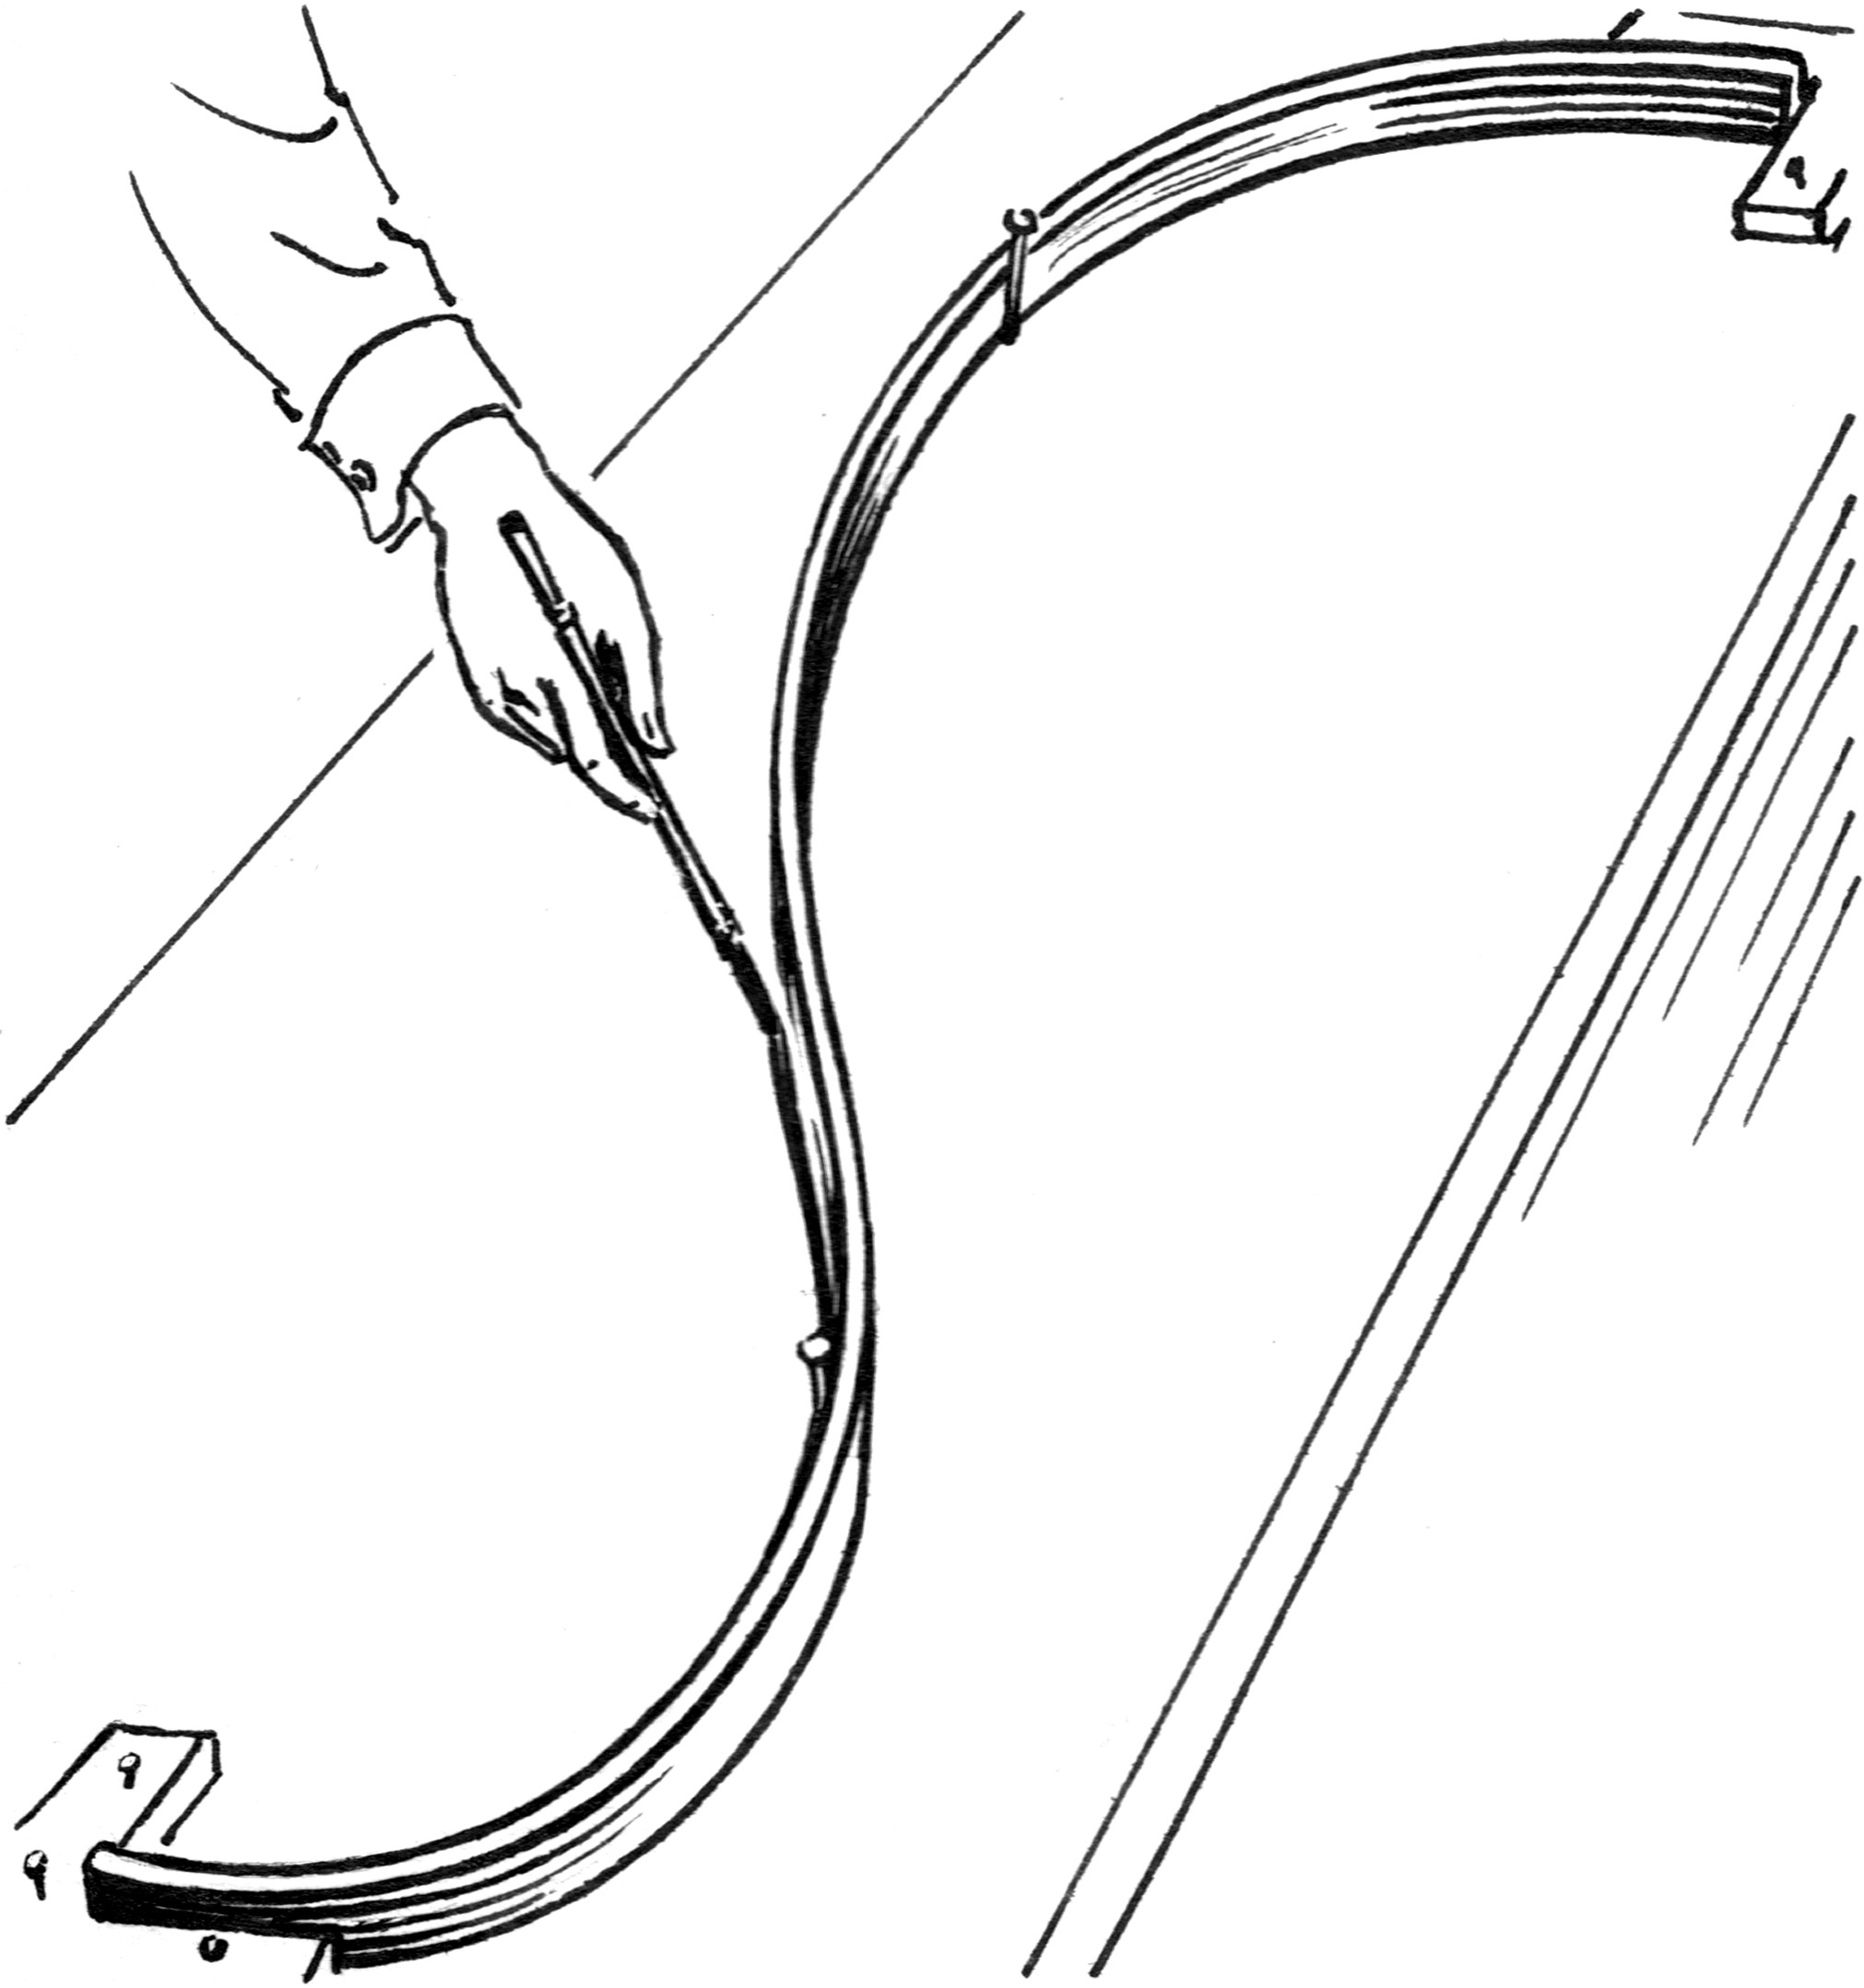
\includegraphics[width= 0.75\linewidth]{8}
			\caption{\small\textit{\color{toanhocdoisong}Cách làm thanh spline khi đóng tàu.}}
			\vspace*{-10pt}
		\end{figure}
		Trước kia, người ta dùng thuật ngữ \textit{spline} để gọi tên thanh gỗ được uốn cong bằng cách kẹp cố định một số điểm. Cách làm này giúp tạo ra đường cong được uốn tự nhiên trong quá trình đóng tàu. Trong toán học, các hàm số có dạng đa thức trên từng đoạn được gọi là các hàm spline. Những đường cong dùng để xấp xỉ sử dụng những hàm spline được gọi là các đường cong spline, bao gồm đường cong Bézier và những đường cong được phát triển sau này dựa trên nó như B--spline, NURB, ... Những đường cong này hiện nay được ứng dụng rộng rãi trong các lĩnh vực công nghiệp như sản xuất máy bay, ô tô, thời trang, ... cũng như trong các lĩnh vực đồ họa máy tính và kiến trúc.
		\vskip 0.1cm
		$\pmb3.$ \textbf{\color{toanhocdoisong}Vẽ đường cong Bézier bằng quỹ tích trong GeoGebra}
		\vskip 0.1cm
		Ta có thể vẽ đường cong Bézier bằng cách nhập phương trình tham số một cách trực tiếp. Tuy nhiên, việc vẽ bằng quỹ tích sẽ mang tính trực quan hơn. Để vẽ đường cong này theo quỹ tích, ta sử dụng cách mô tả của De Casteljau và cho hệ số $k$ thay đổi trong khoảng $[0,1]$. Khi $k=0$, $R$ trùng với $P_0$, còn khi $k=1$, $R$ trùng với $P_1$. Quỹ tích của $R$ chính là đường cong Bézier.
		\vskip 0.1cm
		Trong GeoGebra, trước hết ta chọn các điểm $P_0$, $P_1$ và $P_2$ trong mặt phẳng rồi nối các đoạn thẳng $P_0 P_1$ và $P_1 P_2$.
		\begin{align*}
			&d_1= segment (P_0,P_1)\\
			&d_2= segment (P_1,P_2)
		\end{align*}
		\begin{figure}[H]
			\vspace*{-5pt}
			\centering
			\captionsetup{labelformat= empty, justification=centering}
			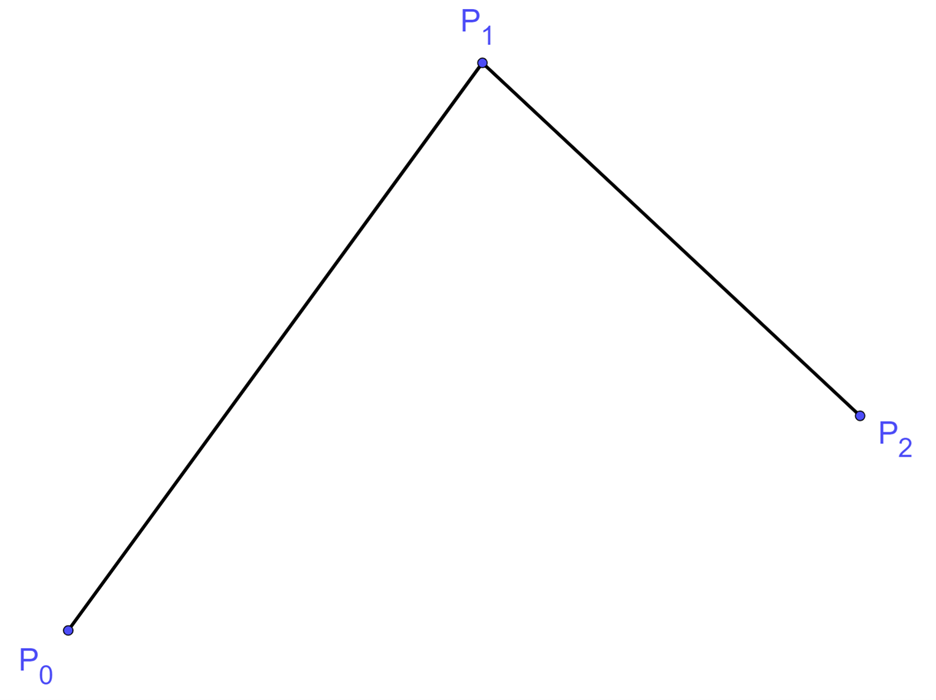
\includegraphics[width= 0.8\linewidth]{9}
			\caption{\small\textit{\color{toanhocdoisong}Hình $5$. Chọn $3$ điểm trong mặt phẳng để xác định đường cong Bézier bậc $2$.}}
			\vspace*{-10pt}
		\end{figure}
		Ta cho tham số $k$ chạy từ $0$ đến $1$:
		\begin{align*}
			k = slider (0,1).
		\end{align*}
		Để xác định các điểm $Q_0$ và $Q_1$, thay vì dùng công thức dạng vector, ta có thể sử dụng giao điểm của đường tròn và đoạn thẳng:
		\begin{align*}
			&Q_0=intersect\left(\text{circle} (P_0,d_1*k),d_1\right)\\
			&Q_1=intersect\left(\text{circle} (P_1,d_2*k),d_2\right)
		\end{align*}
		Điểm $R$ cũng được xác định tương tự:
		\begin{align*}
			&d_3=segment(Q_0,Q_1 )\\
			&R=intersect\left(\text{circle} (Q_0,d_3*k),d_3\right).
		\end{align*}
		Ta ấn chuột phải vào điểm $R$ và chọn ``Show trace''. Khi đó, cho thanh trượt của $k$ di chuyển từ $0$ đến $1$, quỹ tích của $R$ sẽ cho ta đường cong Bézier bậc $2$ (bạn đọc có thể thử chứng minh bằng hình học giải tích rằng nó chính là đường cong này).
		\begin{figure}[H]
			\vspace*{-5pt}
			\centering
			\captionsetup{labelformat= empty, justification=centering}
			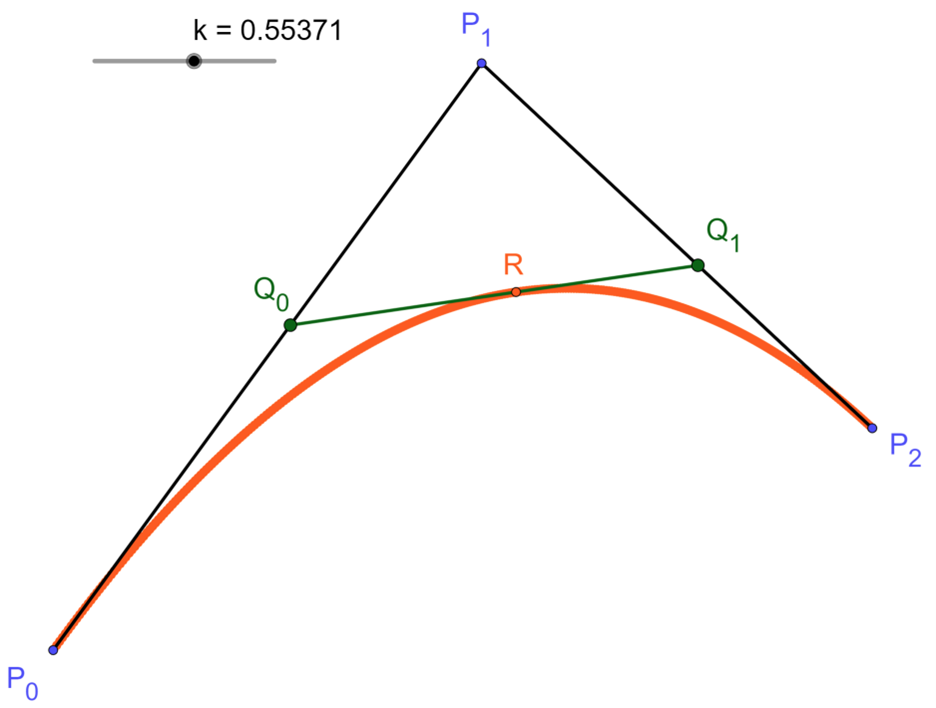
\includegraphics[width= 0.8\linewidth]{10}
			\caption{\small\textit{\color{toanhocdoisong}Hình $6$. Đường cong Bézier bậc $2$ dưới dạng quỹ tích trong GeoGebra.}}
			\vspace*{-10pt}
		\end{figure}
		Với đường cong Bézier bậc $3$, ta sẽ có $4$ điểm $P_0,P_1,P_2$ và $P_3$. Để tiến hành dựng đường cong, ta xác định các điểm $Q_0,Q_1$ và $Q_2$ sao cho $\dfrac{P_0 Q_0}{P_0 P_1}= \dfrac{P_1 Q_1}{P_1 P_2}= \dfrac{P_2 Q_2}{P_2 P_3} =k$. Từ $3$ điểm này, ta lại tiếp tục tìm các điểm $R_1$, $R_2$ và $S$ sao cho $\dfrac{Q_0 R_1}{Q_0 Q_1} = \dfrac{Q_1 R_2}{Q_1 Q_2}= \dfrac{R_1 S}{R_1 R_2}=k$. Quỹ tích của $S$ chính là đường cong cần dựng.
		\begin{figure}[H]
			\vspace*{-5pt}
			\centering
			\captionsetup{labelformat= empty, justification=centering}
			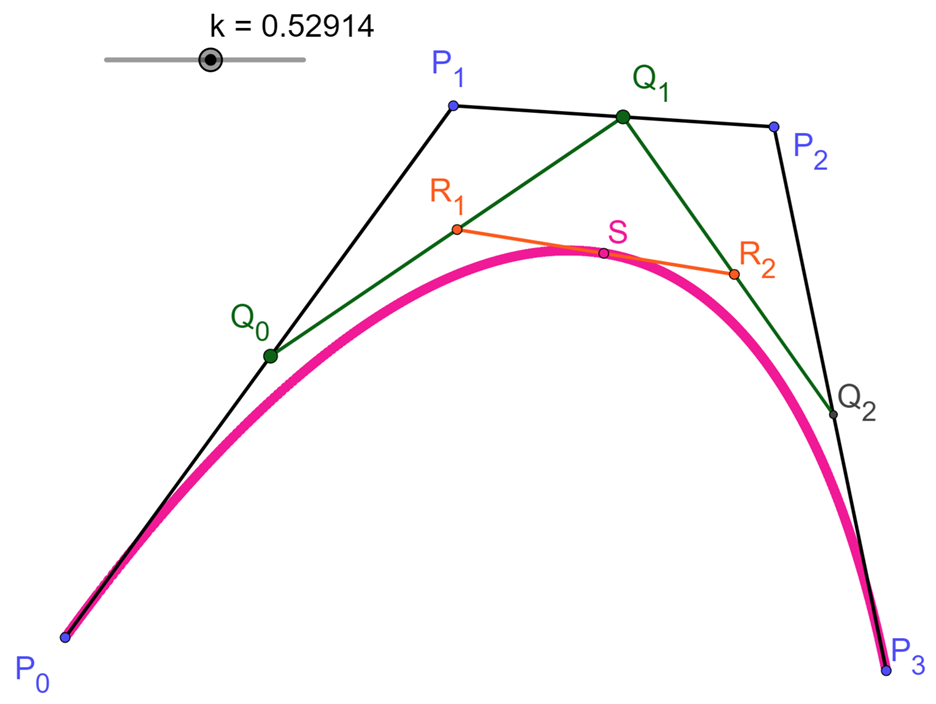
\includegraphics[width= 0.8\linewidth]{11}
			\caption{\small\textit{\color{toanhocdoisong}Hình $7$. Đường cong Bézier bậc $3$ dưới dạng quỹ tích trong GeoGebra.}}
			\vspace*{-10pt}
		\end{figure}
		Với các đường cong Bézier bậc cao hơn, quá trình cũng tương tự, ở mỗi bước ta giảm đi một điểm cho đến khi chi còn lại điểm cuối cùng và tìm quỹ tích của điểm này.
		\vskip 0.1cm
		Cho trường hợp đường cong Bézier bậc $3$, ta có thể thay đổi vị trí các điểm $P_i$ để được các dạng đường cong khác nhau. Có thể thấy, chỉ với tọa độ của vài điểm trong không gian, ta đã có thể xấp xỉ những đường cong phức tạp. Do tính dễ điều chỉnh này mà đường cong Bézier còn được sử dụng để tạo hình động trong đồ họa máy tính. Ta chỉ cần yêu cầu phần mềm thay đổi tọa độ của các điểm điều khiển và toàn bộ đường cong sẽ được di chuyển theo mà không phải đưa ra yêu cầu phức tạp nào khác.
		\begin{figure}[H]
			\vspace*{-5pt}
			\centering
			\captionsetup{labelformat= empty, justification=centering}
			$a)$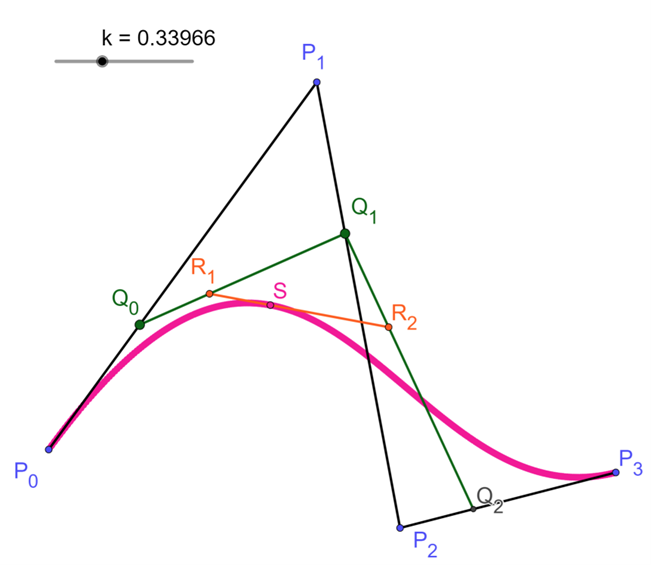
\includegraphics[width= 0.83\linewidth]{12}
			$b)$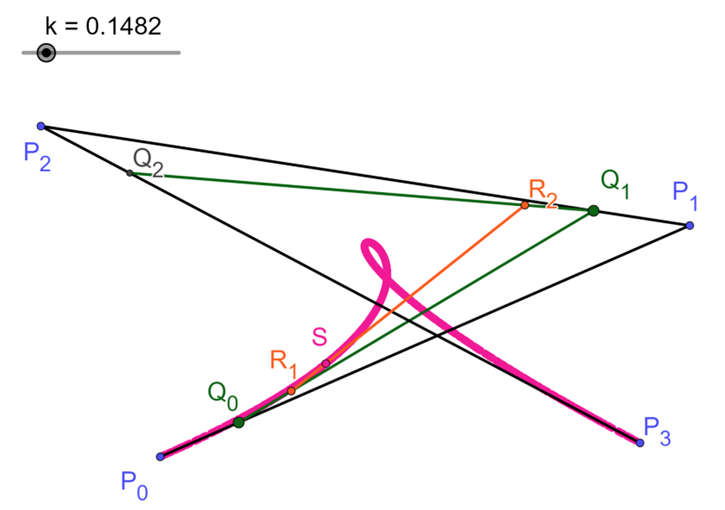
\includegraphics[width= 0.83\linewidth]{13}
			$c)$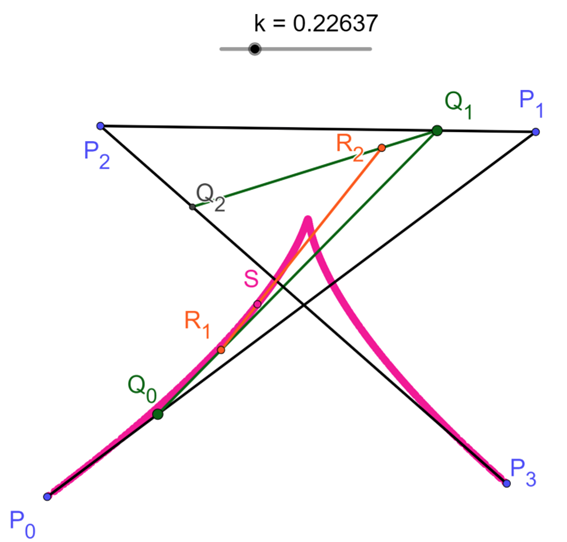
\includegraphics[width= 0.83\linewidth]{14}
			\caption{\small\textit{\color{toanhocdoisong}Hình $8$. Một số dạng đường cong Bézier bậc $3$ khi ta thay đổi vị trí các điểm xác định nó. $a)$ Đường cong có điểm uốn. $b)$ Đường cong có vòng. $c)$ Đường cong có điểm đỉnh.}}
			\vspace*{-5pt}
		\end{figure}
		$\pmb4.$ \textbf{\color{toanhocdoisong}Lời kết}
		\begin{figure}[H]
			\vspace*{-5pt}
			\centering
			\captionsetup{labelformat= empty, justification=centering}
			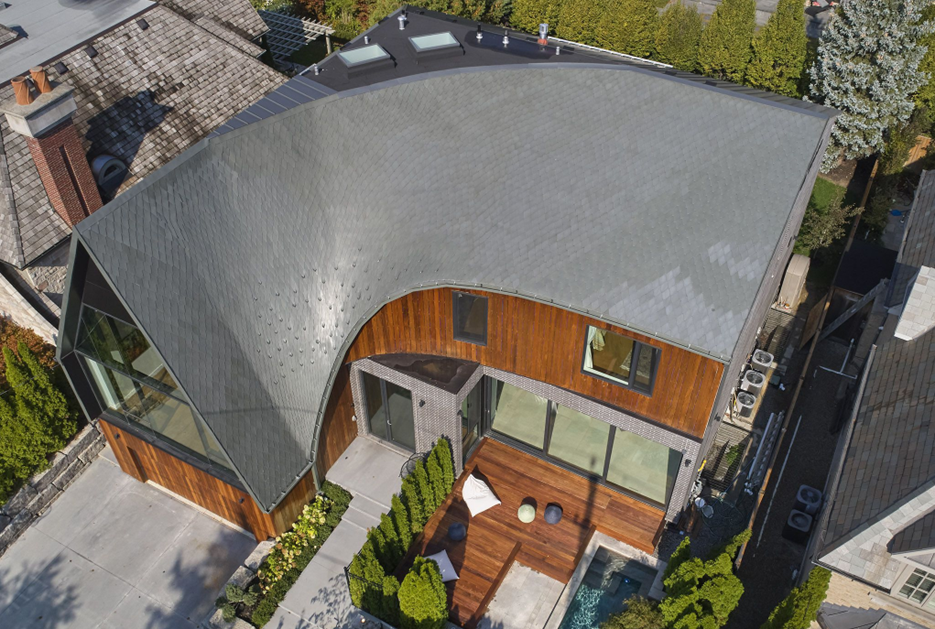
\includegraphics[width= 1\linewidth]{15}
			\caption{\small\textit{\color{toanhocdoisong}Hình $9$. Đường cong Bézier cũng được các kiến trúc sư sử dụng khi thiết kế với sự hỗ trợ của phần mềm. Trong ảnh là một căn nhà có hình dạng mái được thiết kế với đường cong Bézier.}}
			\vspace*{-10pt}
		\end{figure}
		Đường cong Bézier cho thấy ngay cả trong các ngành sản xuất phục vụ đời sống, toán học cũng có thể có những đóng góp quan trọng giúp cải tiến và nâng cao hiệu quả công việc. Toán học được ứng dụng rất phổ biến trong các ngành công nghiệp nhưng vai trò này của nó lại ít được các tài liệu nhắc đến. Việc trình bày về những ứng dụng này học sinh sẽ giúp các em có hứng thú hơn với các lĩnh vực khoa học và công nghệ khi định hướng tương lai cho bản thân. Những đường cong hình học còn có nhiều ứng dụng thú vị khác mà Pi sẽ trình bày trong các số sau này với độc giả.
		\begin{figure}[H]
			\vspace*{-5pt}
			\centering
			\captionsetup{labelformat= empty, justification=centering}
			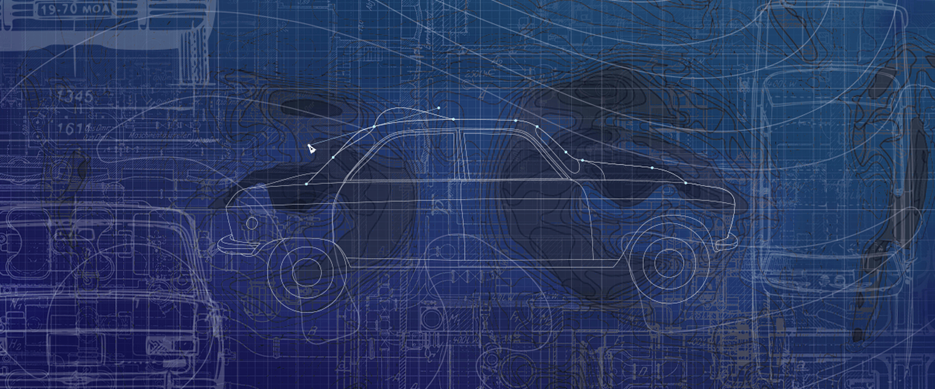
\includegraphics[width= 1\linewidth]{16}
			%		\caption{\small\textit{\color{}}}
			\vspace*{-18pt}
		\end{figure}
		\textbf{\color{toanhocdoisong}Phụ lục:} Chứng minh định lý xấp xỉ Weierstrass sử dụng đa thức Bernstein
		\vskip 0.1cm
		Xét 
		\begin{align*}
			B_n(f,t) &= \sum\limits_{i = 0}^n {f\left( {\frac{i}{n}} \right)B_i^n(t)}  \\
			&= \sum\limits_{i = 0}^n {\left( \begin{array}{l}
					n\\
					i
				\end{array} \right){{(1 - t)}^{n - i}}{t^i}f\left( {\frac{i}{n}} \right)}.
		\end{align*}
		Với $t\in [0,1]$, ta có:
		\begin{align*}
			&|f(t) - B_n(f,t) \\
			= &|\left(t + (1-t)\right)^nf(t) - B_n(f,t)|\\
			=&\left| {\sum\limits_{i = 0}^n {B_i^n(t)}  = \left( {f(t) -  - f\left( {\frac{i}{n}} \right)} \right)} \right|\\
			\le &\sum\limits_{i = 0}^n {\left( \begin{array}{l}
					n\\
					i
				\end{array} \right){{(1 - t)}^{n - i}}{t^i}} \left| {f(t) - f\left( {\frac{i}{n}} \right)} \right| = S
		\end{align*}
		\begin{figure}[H]
			\vspace*{-5pt}
			\centering
			\captionsetup{labelformat= empty, justification=centering}
			$a)$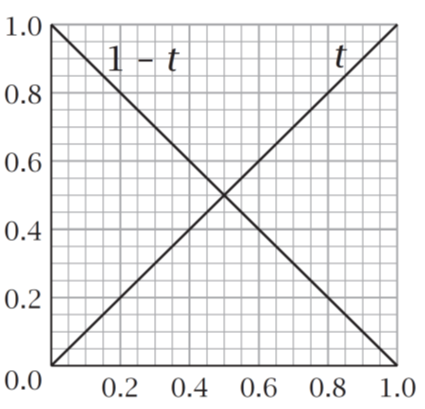
\includegraphics[width= 0.77\linewidth]{17}
			$b)$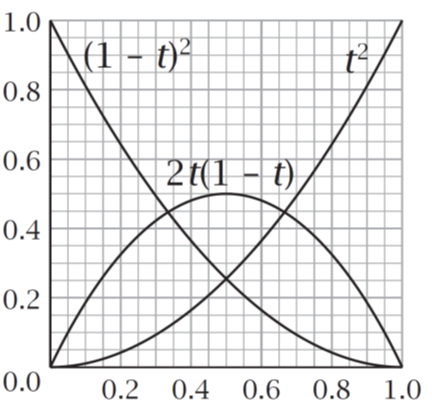
\includegraphics[width= 0.77\linewidth]{18}
			\hspace*{15pt}$c)$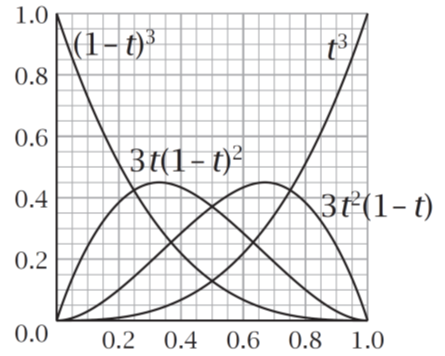
\includegraphics[width= 0.89\linewidth]{19}
			\caption{\small\textit{\color{toanhocdoisong}Hình $9$. $a)$ Các đa thức Bernstein bậc $1$. $b)$ Các đa thức Bernstein bậc $2$. $c)$ Các đa thức Bernstein bậc $3$.}}
			\vspace*{-5pt}
		\end{figure}
		Quan sát đồ thị của các $B_i^n (t)$, ta nhận thấy đỉnh của chúng sẽ gần với một giá trị $t= \dfrac{i}{n}$ và phần lớn diện tích dưới đường cong sẽ phân bố xung quanh đỉnh này. Điều đó có nghĩa rằng các hàm số Bernstein có $\dfrac{i}{n}$ gần với $t$ hơn sẽ có đóng góp nhiều hơn cho $B_n (f,t)$. Do đó, ta có thể tách $S$ thành hai phần như sau với $ \delta >0$:
		\begin{align*}
			S =& \sum\limits_{\left| {\frac{i}{n} - t} \right| \ge \delta }\!\!\! \left(\!\!\!\! \begin{array}{l}
				n\\
				i
			\end{array}\!\!\!\! \right){{(1 \!-\! t)}^{n - i}}{t^i}\left| {f(t) - f\left( {\frac{i}{n}} \right)} \right| \\
			&+ \!\! \sum\limits_{\left| {\frac{i}{n} - t} \right| < \delta }\!\!\! \left(\!\!\!\! \begin{array}{l}
				n\\
				i
			\end{array}\!\!\!\! \right){{(1 \!-\! t)}^{n - i}}{t^i}\left| {f(t) \!-\! f\left(\! {\frac{i}{n}} \!\right)} \right|\\
			=&\,\, S_1 + S_2.
		\end{align*}
		Tiến hành khai triển đại số và sử dụng một số công thức để biến đổi tổ hợp, ta có các công thức sau:
		\begin{align*}
			&\sum\limits_{i = 0}^n {B_i^n(t) = 1}.\\
			&\sum\limits_{i = 0}^n {i \cdot B_i^n(t) = nt.}\\
			&\sum\limits_{i = 0}^n {i(i - 1) \cdot B_i^n(t) = n(n - 1){t^2}.}
		\end{align*}
		Từ ba công thức này ta có:
		\begin{align*}
			&\sum\limits_{i = 0}^n {{{(i - nt)}^2}B_i^n(t)} \\
			=\,\, &\sum\limits_{i = 0}^n \left[ {i(i - 1) - (2nt - 1)i + {n^2}{t^2}} \right]B_i^n \\
			= \,\,&n(n - 1){t^2} - (2nt - 1)nt + {n^2}{t^2} \\
			= \,\,&nt(1 - t) \le \frac{n}{{4.}}
		\end{align*}
		Chia cả hai vế cho $n$ ta được:
		\begin{align*}
			\sum\limits_{i = 0}^n {{{\left( {\frac{i}{n} - x} \right)}^2}B_i^n(t) \le \frac{1}{{4n}}.}
		\end{align*}
		Do đó:
		\begin{align*}
			\sum\limits_{\left| {\frac{i}{n} - t} \right| \ge \delta } {B_i^n(t)} &\le  \frac{1}{{{\delta ^2}}}\sum\limits_{\left| {\frac{i}{n} - t} \right| \ge \delta } {{\left( {\frac{i}{n} - t} \right)}^2}B_i^n(t) \\
			&\le \frac{1}{{{\delta ^2}}} \cdot \frac{1}{{4n}}.
		\end{align*}
		Với giá trị $M$ thỏa mãn $|f(t)| \le M$ trên $[0,1]$, ta có:
		\begin{align*}
			{S_1} &\le \sum\limits_{\left| {\frac{i}{n} - t} \right| \ge \delta } \left| {f(t) - f\left( {\frac{i}{n}} \right)} \right|B_i^n(t) \\
			&\le 2M \cdot \frac{1}{{4n{\delta ^2}}} = \frac{M}{{2{\delta ^2}n}}.
		\end{align*}
		Với một giá trị $\epsilon$ cho trước, với $\delta$ đủ nhỏ sao cho $|f(u)-f(v)| \le \dfrac{\epsilon}{2}$ khi $|u-v|< \delta$ trong khoảng $[0,1]$, ta có:
		\begin{align*}
			{S_2} \le \sum\limits_{\left| {\frac{i}{n} - t} \right| \ge \delta } {\frac{\epsilon}{2} \cdot B_i^n(t)}  < \frac{\epsilon}{2}\sum\limits_{i = 0}^n {B_i^n(t) = \frac{\epsilon}{2}}.
		\end{align*}
		Tóm lại, với $\epsilon>0$ cho trước và $\delta$ thỏa mãn điều kiện nêu ở trên, khi $n$ đủ lớn để $\dfrac{M}{2\delta^2n} < \dfrac{\epsilon}{2}$, ta có:
		\begin{align*}
			|f(x)- B_{n,f}(t)| < \dfrac{\epsilon}{2} + \dfrac{\epsilon}{2} = \epsilon.
		\end{align*}
		Thay vì biến đổi sử dụng các công thức tổ hợp, ta cũng có thể sử dụng bất đẳng thức Chebyshev trong xác suất để chứng minh $S_1 \le \dfrac{M}{2\delta^2n}$. Bất đẳng thức Chebyshev được phát biểu như sau: Cho $p$ là một phân phối rời rạc với giá trị trung bình $m$ và độ lệch chuẩn $\sigma$, khi đó: $P(|x-m| \ge s \cdot \sigma) \le \dfrac{1}{s^2}$ (chứng minh của bất đẳng thức này không quá phức tạp và có thể được tìm thấy trong các giáo trình xác suất hoặc qua internet). Với trường hợp của ta, $B_i^n (t)$ là các giá trị ứng với $p(x=i)$ của phân phối nhị thức có trung bình là $m=nt$. Độ lệch chuẩn tương ứng của phân phối này sẽ là $\sigma = \sqrt{nt(1-t)}$. Theo bất đẳng thức Chebyshev, chọn $s$ sao cho $s \cdot \dfrac{\sigma}{n} = \delta$, ta có:
		\begin{align*}
			&P\left(|x- nt| \ge s \cdot \sigma\right)\\
			= \,\,&\sum\limits_{\left| {\frac{i}{n} - t} \right| \ge \delta } {B_i^n(t)}  \le \frac{1}{{{s^2}}} \\
			= \,\,&\frac{{{\sigma ^2}}}{{{n^2}{\delta ^2}}} = \frac{{t(1 - t)}}{{n{\delta ^2}}} \le \frac{1}{{4n{\delta ^2}}}.
		\end{align*}
		\textbf{\color{toanhocdoisong}Tài liệu tham khảo}
		\vskip 0.1cm
		[$1$] Farin, Gerald. \textit{Curves and Surfaces for Computer--Aided Geometric Design}. Elsevier, $28$ June $2014$.
		\vskip 0.1cm
		[$2$] Farin, Gerald E, et al. \textit{Handbook of Computer Aided Geometric Design}. Amsterdam ; Boston, Mass., Elsevier, $2002$.
		\vskip 0.1cm
		[$3$] Havil, Julian. \textit{Curves for the Mathematically Curious : An Anthology of the Unpredictable, Historical, Beautiful and Romantic}. Princeton, New Jersey ; Oxford, Princeton University Press, $2019$.
		\vskip 0.1cm
		[$4$] Levasseur, Kenneth M. ``A Probabilistic Proof of the Weierstrass Approximation Theorem.'' T\textit{he American Mathematical Monthly}, vol. $91$, no. $4$, Apr. $1984$, p. $249$, \url{https://doi.org/10.2307/2322960}. Accessed $31$ Oct. $2019$.
		\vskip 0.1cm
		[$5$] Salomon, David. \textit{Curves and Surfaces for Computer Graphics}. New York, Ny, Springer New York, $2006$.
	\end{multicols}